\documentclass[tog]{acmsiggraph}
\graphicspath{{./images/}}
\usepackage{gensymb}
\usepackage[ngerman]{babel}
\usepackage[utf8]{inputenc}
\usepackage[T1]{fontenc}
\usepackage{hyperref}
\usepackage{listings}
\newcommand{\code}[1]{\texttt{#1}}
%%% Make the ``BibTeX'' word pretty...
\def\BibTeX{{\rm B\kern-.05em{\sc i\kern-.025em b}\kern-.08em
    T\kern-.1667em\lower.7ex\hbox{E}\kern-.125emX}}

%%% Used by the ``review'' variation; the online ID will be printed on 
%%% every page of the content.

\TOGonlineid{00001}

%%% Used by the ``preprint'' variation.

\TOGvolume{0}
\TOGnumber{0}

\title{Übung 1 - Computergrafik-I, WS 2015/16}
\author{Christoph Stumpe, Fabian Wendland, Martin Zier\\Beuth Hochschule für Technik Berlin}
\pdfauthor{Martin Zier, s59330}
\date{25. Oktober 2015}

\keywords{Matrizen, Mathematik, Java Übung}

\begin{document}
 \teaser{
   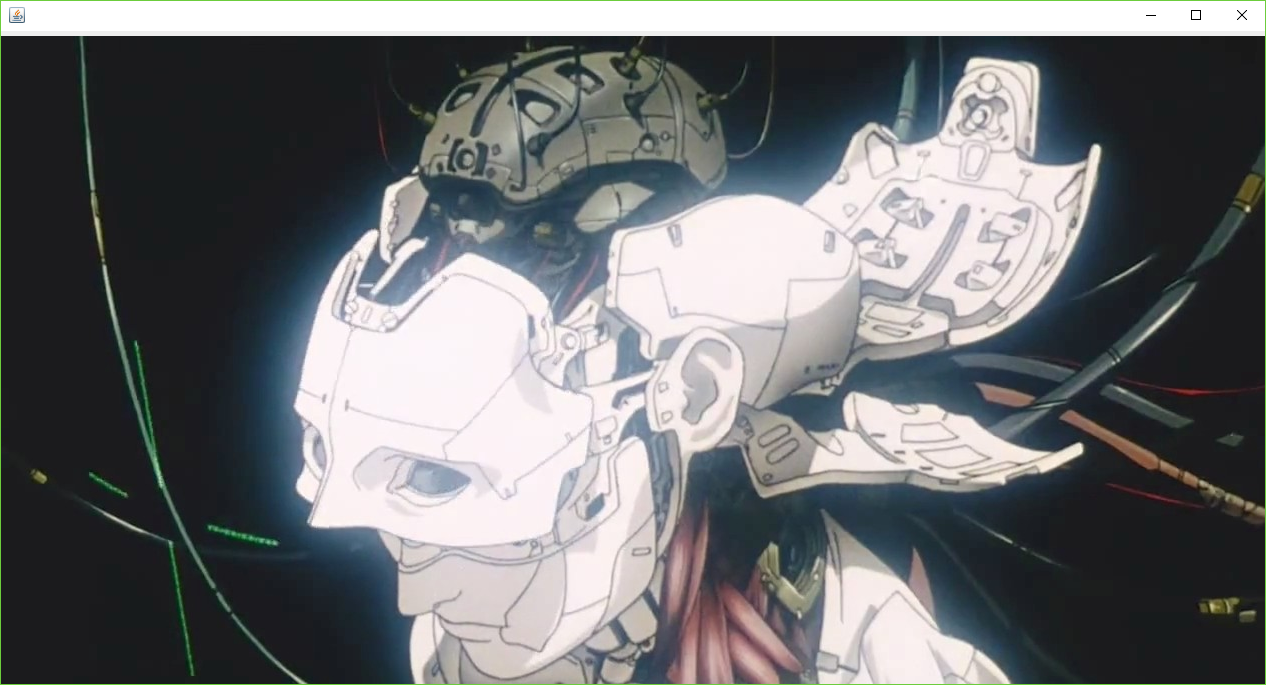
\includegraphics[height=2in]{01_image-frame.png}
   \caption{Vorbereitungsübung 1 -- Quelle: \textsc{Ghost in the Shell}, 1996}
 }
\maketitle

\tableofcontents
\newpage

\section{Einführung}

In der Vorbereitung werden Grundkenntnisse überprüft und dienen zur Wiederholung der objektorientierten Programmierung. Außerdem wird auf dem vorbereiteten Quellcode aufgebaut und programmiert.

\section{Aufgabenstellung}

Alle dargestellten Aufgaben beziehen sich auf die Implementierung mit Java sofern nicht anders gekennzeichnet.

\subsection{Bilddarstellung \& -generierung}

Es werden zwei verschiedene Programme gefordert:

\begin{itemize}
\item \textbf{Bilddarstellung}: Ein Programm, welches nach dem Pfad einer Bilddatei fragt und diese dann in einem Fenster anzeigt.
\item \textbf{Bildgenerierung}: Ein Programm, welches in einem Fenster mit schwarzem Grund eine rote Linie im 45\degree Winkel zeigt. Der gezeigte Inhalt entspricht der Fenstergröße und muss gegebenenfalls nachgezeichnet werden, wenn die Fenstergröße verändert wird. Dieses generierte Bild soll in seiner aktuellen Rendergröße zu speichern sein --- das bedeutet ebenfalls, dass bei veränderter Größe das gespeicherte Bild sich in Größe und Proportion verändert.
\end{itemize}

\subsection{Grundlegende Vektormathematik}
\label{mathTemplate}
Die mathematischen Implementierungen werden wie folgt gefordert\footnote{Jedes Element
der Auflistung bezieht sich auf ein einzelnes Objekt in eigener Klasse.}:

\begin{itemize}
\item \textbf{Normal3}: Eine Normale mit x, y, z Koordinate. \newline
						Ebenfalls soll sie mit einer Normale multipliziert und addiert
						werden können. \newline Außerdem soll das Skalarprodukt mit einem
						\textit{Vector3} möglich sein.
\item \textbf{Point3}: Ein Punkt mit x, y, z Koordinate. \newline
						Es soll möglich sein einen \textit{Point3} mit einem
						\textit{Vector3} zu addieren und zu subtrahieren. Das
						Ergebnis ist ein neuer \textit{Point3}. \newline Außerdem ergibt
						die Subtraktion mit einem \textit{Point3} einen neuen
						\textit{Vector3}.
\item \textbf{Mat3x3}: Eine 3x3 Matrix, die über einen vollständigen Konstruktor
						initialisiert wird. Zusätzlich soll die Determinante bei
						Initialisierung bestimmt werden, falls nicht mit dem Konstruktor
						aufgerufen.
						\newline Diese Matrix soll Methoden haben um einzelne
						Zeilen (mittels eines \textit{Vector3}) auszutauschen. \newline
						Zusätzlich sollen folgende Matrixmultiplikationen möglich sein
						\footnote{Matrix :: Eingabe >> Ausgabe}:
						\begin{enumerate}
						\item \textbf{Mat3x3} :: \textit{Mat3x3} >> \textit{Mat3x3}
						\item \textbf{Mat3x3} :: \textit{Vector3} >> \textit{Vector3}
						\item \textbf{Mat3x3} :: \textit{Point3} >> \textit{Vector3}
						\end{enumerate}
\end{itemize}

\subsection{Pythonimplementierung}

Wir haben uns entschieden den Basis-Raytracer in Python zu portieren. Bis zur Erstellung dieses Papiers ist noch nicht endgültig entschieden ob wir das Render-Backend in C (mit Python-Bindings) programmieren oder gar in Assembler schreiben. Allein der Geschwindigkeit wegen, wird es sich im späteren Verlauf als sinnvoll darstellen, dass alle einfachen mathematischen Objekte in C implementiert werden und die Python-Portierung nur noch die dazugehörigen API offengelegt wird. \newline
Die bisherige Implementation wird den advanced Python-Syntax verwenden, indem wir z. B. die Standardoperatoren von Python-Objekten überschreiben. \newline

Die Debug-Output aller Objekte und der notwendigen Funktionen wird gespiegelt zur Java-Implementierung programmiert. Dabei werden ggf. Segmente so portiert, dass syntaktisch und funktional alle Richtlinen der PEP8\footnote{\url{https://www.python.org/dev/peps/pep-0008/}} eingehalten werden.

\subsection{Addendum}

Die Klassen werden durch Akzeptanzkriterien der vorliegenden Aufgaben geprüft. Diese Akzeptanzkriterien können im Aufgabenblatt zu diesem Papier nachgesehen werden. Eine Kopie der Aufgaben ist auf der Seite von \footnote{\url{http://rehfeld.beuth-hochschule.de/2015-ws-cg1.html}} erhältlich. Unittests werden nicht geschrieben.

Der dazugehörige Python-Code wird durch die selbigen Akzeptanzkriterien geprüft.

\section{Lösungsstrategien}

Die Vorbereitungsaufgaben benötigten keine gesonderten Strategien. Unsere Übungsgruppe hat sich darauf geeinigt, zunächst einen eigenen Branch anzulegen und die Vorbereitungsaufgaben selbst zu implementieren. Dadurch können nach der Semesterpause noch einmal die Kenntnisse aufgefrischt werden und die Aufgaben stellen ein Mindestmaß des bisherigen Grundstudiums dar.

\newpage
\section{Implementierung und Bearbeitungszeit}

Die Java-Implementierung versucht alle Code-Conventions einzuhalten und entspricht der Aktualität zur Übungsabgabe. Diese Implementierung wird nach bestem Wissen und Gewissen zu dem Zeitpunkt der Abgabe von den Studenten programmiert.

\subsection{Bilddarstellung}

Bei der Implementierung kann ein einfaches, unmodifiziertes \code{JOptionPane} verwendet werden. Nach der Initialisierung aus der Auswahl des \code{JOptionPane} wird eine Gegenprobe auf den Dateityp durchgeführt --- mithilfe von \code{java.nio.file.Files.probeContentType}. Es wird ein \textit{MIME}-String ausgegeben, anhand dessen herausgefunden werden kann, ob es sich um eine Bilddatei handelt. Danach wird das Bild in ein \code{BufferedImage} geladen und in einem \code{JFrame} angezeigt.

\textbf{Bearbeitungszeit}: 0,5 -- 1,5 Stunden

\subsection{Bildgenerierung}

Ein \code{JFrame} erzeugt ein \code{ImagePanel}. Dieses \code{ImagePanel} ist ein modifizierted \code{JPanel} welches eine rote Linie im 45\degree Winkel erzeugt --- die Bildinformationen werden in einem \code{BufferedImage} gespeichert. Durch die Implementierungsform von \code{BufferedImage} ist die erzeugte Bildinformation grundsätzlich schwarz. Diese Gegebenheit lässt sich dadurch ausnutzen, dass für die Liniengenerierung nur noch das größere Maß von Höhe und Breite definiert werden muss und erhält dadurch eine Laufzeit von $\mathcal O(n) $\footnote{\code{max(height, width)}} statt $\mathcal O(n_{h}*n_{w}) $\footnote{\code{height * width}}.

\textbf{Bearbeitungszeit}: 1,0 -- 1,5 Stunden

\subsection{Vektormathematik}

Die Implementierung erfolgt nach den Richtlinien aus \ref{mathTemplate}. Die Implementierung ist simpel und geradlinig nach den UML-Diagrammen aus der Aufgabenstellung programmiert.

\textbf{Bearbeitungszeit}: 2,0 -- 2,5 Stunden

\subsection{Pythonimplementierung}

Wie vorher bereits erwähnt, erfolgt die Implementierung mit ähnlicher Objekt-API wie der Java-Implementation. Zwar werden Objekt-Operationen überschrieben, allerdings werden auch darauf Operationen auf diese Objekt-Methoden weitergeleitet: \newline

\lstset{language=Python} 
\begin{lstlisting}

class Object:
	def __mul__(self, other):
		pass
	def mul(self, other):
		return self * other

\end{lstlisting}

Dadurch wird der Portierungsvorgang im späteren Verlauf erheblich vereinfacht, da nicht alle Funktionsaufrufe neu geschrieben werden müssen und unübersichtliche Rechnungen können erheblich verkürzt werden.

\textbf{Bearbeitungszeit}: 2 Stunden

\section{Aufgetretene Probleme der Implementierung}

\begin{itemize}
	\item \textbf{\LaTeX - Einarbeitung, Einrichtung}:\newline
			LaTeX stellt eine ungeheure Herausforderung dar, hauptsächlich da keine empfohlenden Tools vorgestellt wurden. Die Arbeit ist allen beteiligten Studenten neu.
\end{itemize}

\section{Quellen \& Literaturverzeichnis}

\begin{itemize}
	\item \url{https://asalga.wordpress.com/2012/09/23/understanding-vector-reflection-visually/}
	\item \url{http://geomalgorithms.com/points_and_vectors.html#Vector-Addition}
	\item \url{http://docs.oracle.com/javase/8/docs/api/}
	\item Fundamentals of Computer Graphics -- \textsc{Peter Shirley \& Steve Marschner}
\end{itemize}

\end{document}
